\documentclass[12pt]{article}
\usepackage{url}
\usepackage{graphicx}
\graphicspath{ {/}}


\title{Fairbook: DIS}

\author{A. Snow, C. McKenzie, C. Yang, J. Lyons, M. Zhang}

\begin{document}
	\maketitle


	\tableofcontents
	\section{ONIDs}
		snowan, mckencod, yangco, lyonsja, zhangm4



	\section{UML Class Diagram}
	\includegraphics[width=16cm]{uml_class_diagram.ps}


	\section{Packages}
First of all, the main page of the website of Fairbook is simply implemented by a .html files and decorated by a .css files. The function of adding textbook and purchasing will be implemented in a .js file.
For the search bar, we will make a function for it to search the existing textbooks by names which inputted by users. For the search filter, we will make a function to let user change the checked status of given information so that user can find the textbooks that come with the information they want to know.
The name, subject, condition and price will be written in the classes of corresponding textbooks, besides displayed to the user. In this way, we can use filter to search for desired textbook according to the value of corresponding class.
Each div of individual textbook stays in the section of textbooks. When we move to dynamic data, we may use database such as MongoDB to store our data.
So far, I don’t have clear concept of implementing the authorization part yet, and we will try to figure it out as we move on.
In overall, the structure of our implementation will have high cohesion which gives good quality of clarity and understanding, and loose coupling which reduces the difficulties to make change to part of project.



	\section{Design Patterns}

We believe our project would fall in the line of Interpreter, Observer and Decorator patterns.  
The reason I believe our project would be in the Decorator pattern is because a website has to have a general look to it that is seperate from some of the functions we program.  
Our project also falls into the Interpreter pattern because we have to be able to take the clicks and inputs of users more than anything else on the site, the clicks and input will tell the site where to go and give details  on the stuff customers want to buy or sell.  
The Observer pattern also fits because we need to observe when a seller adds or removes a book they are selling, this will also notify a seller if a customer is interested in the book they are selling.  
Likewise it can notify the user that wants to buy a book that the purchase was successful and he should expect the book to be theirs.  
These three seem to be the best patterns for our book selling website, it is all we will really require to do all the functions and activities we need for our customers.


	\section{Exceptions \& Handling}


	\subsection{Exception 1: No match for searching}
 	\textbf{Description:}
 When user search a particular book, it is possible there is no match, and if the app try to display the result and there is null, it may cause a situation about divide zero and make an error: out of boundary.

	\textbf{Handling:}
When app try to display searching result, check if the result is zero, if not, behaving normally, if it is, show information: there is no such books.
 
	\subsection{Exception 2: Repeat purchases}

	\textbf{Description:}
When user try to buy a book, it may occur that he or she clicks more than once the confirm button and cause more than once purchase.

	\textbf{Handling:}
For this situation, the app could modify to only accept one purchase at a time. Also, it allows user to cancel order if the book is not shipped.
 
	\subsection{Exception 3: Book exist in more than one catalog}

	\textbf{Description:}  
A book may exist in more than one catalog for there is one or more supplier offer the book and they fill out different information. This may cause error then the app tries to display the information stored in different catalog.

	\textbf{Handling:}
The information displayed should in ordered based on the sequence of the catalog, and it search in one catalog, it should not search other catalog in the same time.




	\section{Meeting Report}
	\subsection{Progress Made}

This week, we met up to discuss the project. 
We spent a good portion of the meeting evaluating the requirements in the rubric and determining which member(s) would work on each section. 
We decided that each member would handle one section and then those that wanted to present could collaborate on the slides. 
Not all members were able to meet up in person, but we kept everyone informed via our group text. 
We are continuing with our usage of google drive for all of the design documents. 
Also, we are considering a few different tools/frameworks for when we begin our implementation phase: Google Web Designer mainly.



\subsection{Plans/Goals for Next Week}

Next week’s assignment has not been posted yet. However, we expect that we will begin coding the web application soon. We will likely meet up again on Friday of next week as we have done in the past. We will most likely utilize our scheduling information from prior assignments to help structure the order we will follow when coding each section of our web app.




\subsection{Contributions of Each Member}

\quad Design Patterns--Cody \par
Exceptions and Handling--Mingyu \par
Meeting Report--Jacob \par
Packages--Cong \par
UML Class Diagrams--Andrew \par
PowerPoint--Andrew, Cody, Jacob \par
LaTeX--Jacob

	\end {document}
	
